% Provenance (never printed): old premiere S material on the oceanic lithosphere
% (ophiolite-type layering, peridotite and gabbro, partial melting by decompression
% at the ridge, hydrothermalism, cooling and subsidence of the lithosphere with
% age); see sources/book2/PROVENANCE.md. Melting from figdata/grade-11/
% ridge_melting.py (adiabat and Hirschmann solidus), depth against age from
% depth_age.py (ETOPO1 and the Seton 2020 age grid). Partial melting is re-founded
% in Year 2 (mantle-melting); fault is Book 1's (g7), normal fault is defined here.
\chapter{الظهرات المحيطية والغلاف الصخري المحيطي}\label{ch:g11:ocean-ridges}

في فبراير 1977 صوّرت زلاجة كاميرا مسحوبة على عمق 2500 متر فوق صدع
غالاباغوس، في شرق المحيط الهادئ، اللابة السوداء العارية للظهرة
لقطةً بعد لقطة. ثم سجل مقياس حرارتها ارتفاعًا طفيفًا في
درجة حرارة الماء، وظهرت اللابة في الصور مغطاة
بمئات من المحار الأبيض. وبعد أيام قليلة نزلت الغواصة \emph{«ألفين»}
بجيولوجيين اثنين إلى الموضع: كان ماء دافئ متلألئ يتدفق من
شقوق اللابة، وحوله تعيش محارات بطول الساعد،
وبلح بحر وسرطانات بيضاء؛ وفي غطسة لاحقة، ديدان أنبوبية ذات رؤوس حمراء. ولم يكن أحد
يتوقع وجود حياة هناك، فلم يكن على متن السفينة أي عالم أحياء. يشرح هذا الفصل
ما وجده الجيولوجيان: كيف يُصنع قاع المحيط عند الظهرات،
ولماذا يكون ساخنًا هناك، وماذا يصير إليه وهو يبتعد.
% ledger: whoi:alvin-1977

\begin{recall}
عند الظهرات يُصنع قاع محيطي جديد ويبتعد على الجانبين، فيزداد
عمره مع البعد عن المحور؛ وتشكّل الظهرات منظومة طولها نحو
\qty{65000}{km}، مع وادي خسف على امتداد الظهرات البطيئة وقمة ملساء
على امتداد السريعة (\cref{ch:g11:drift-to-spreading}). وتتباعد الصفائح عبر
الظهرة بضعة سنتيمترات في السنة، أسرع عبر ظهرة شرق المحيط الهادئ منها
عبر ظهرة وسط الأطلسي (\cref{ch:g11:plate-motions}). \omterm{def:g11:lithosphere-asthenosphere:lithosphere}{والغلاف الصخري}
هو الغلاف الخارجي الصلب، \omterm{def:g11:lithosphere-asthenosphere:lithosphere}{والغلاف اللدن} الذي تحته ينساب؛ ولا ترتفع درجة حرارة
\omterm{def:g11:lithosphere-asthenosphere:lithosphere}{الغلاف اللدن} إلا بنحو \qty{0.45}{\celsius} لكل كيلومتر
من العمق، ودرجة انصهار صخر الوشاح ترتفع مع العمق
(\cref{ch:g11:lithosphere-asthenosphere}). والصهارة صخر منصهر تحت
السطح، والبازلت هو الصخر الداكن الذي تكوّنه اللابة حين تبرد، والصدع
كسر تحركت الصخور على امتداده (الكتاب 1، الصفان 6 و7).
\end{recall}
% ledger: noaa:ridge, katsura10:adiabat, hirschmann:solidus

\section{الغلاف الصخري المحيطي}

صخران نادران على سطح القارات يكوّنان معظم
\omterm{def:g11:ocean-ridges:oceanic-lithosphere}{الغلاف الصخري المحيطي}.

\begin{definition}[البيريدوتيت]\label{def:g11:ocean-ridges:peridotite}
\emph{البيريدوتيت}\index{بيريدوتيت} صخر داكن خشن الحبيبات يتكون
في معظمه من معدن الأوليفين، مع شيء من البيروكسين. وهو عادة أخضر
وكثيف. ويُعتقد أن جزءًا كبيرًا من وشاح الأرض مصنوع من البيريدوتيت.
\end{definition}

\begin{definition}[الغابرو]\label{def:g11:ocean-ridges:gabbro}
\emph{الغابرو}\index{غابرو} صخر ناري داكن خشن الحبيبات يتكون
أساسًا من فلسبار البلاجيوكليز والبيروكسين. وله تركيب
البازلت نفسه، لكنه تبلور ببطء، في أعماق باطن الأرض، فأتيح لبلوراته
الوقت لتنمو. وهو أوفر صخور \omterm{def:g11:ocean-ridges:oceanic-lithosphere}{القشرة المحيطية} العميقة.
\end{definition}
% ledger: geo:peridotite, geo:gabbro

المعادن المذكورة هنا، الأوليفين والبيروكسين والفلسبار، موصوفة في
\cref{ch:g11:minerals}.

\begin{omfigure}
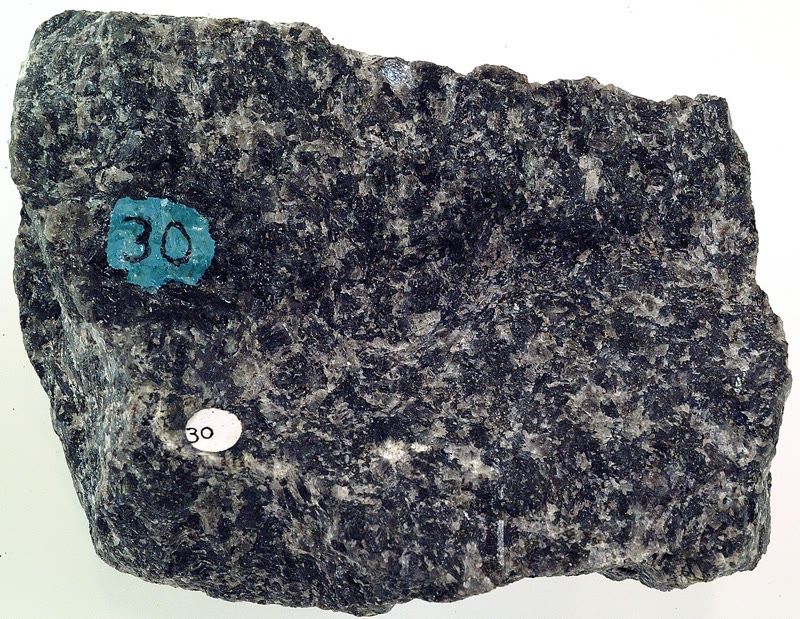
\includegraphics[height=4.2cm]{images/book2/g11-geodil-gabbro.jpg}\hspace{0.03\linewidth}%
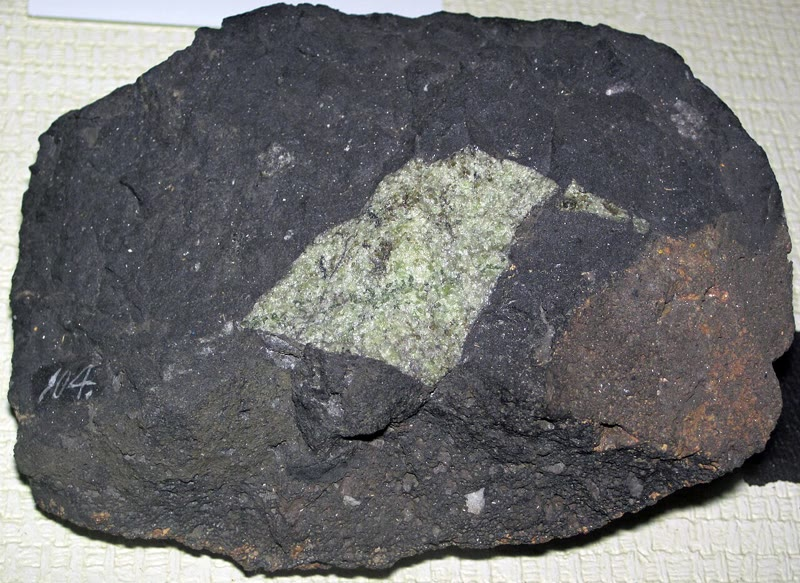
\includegraphics[height=4.2cm]{images/book2/g11-stjohn-peridotite.jpg}

{\small في اليمين: \omterm{def:g11:ocean-ridges:gabbro}{الغابرو}، وعرضه \qty{9}{cm}، وفيه بلورات بيروكسين داكنة وبلورات
فلسبار فاتحة كبيرة بما يكفي لتُرى؛ الصورة: دارلا سوندرول (\babelsublr{CC0}).
في اليسار: كتلة من \omterm{def:g11:ocean-ridges:peridotite}{البيريدوتيت} الأخضر آتية من الوشاح، حملتها إلى الأعلى
لابة بازلت سوداء لبركان في أريزونا؛ الصورة: جيمس سانت~جون (\babelsublr{CC~BY~2.0}).}
\end{omfigure}
% ledger: photo:g11-gabbro, photo:g11-peridotite

\begin{definition}[القشرة المحيطية؛ الغلاف الصخري المحيطي]\label{def:g11:ocean-ridges:oceanic-lithosphere}
\emph{القشرة المحيطية}\index{قشرة محيطية} هي قشرة قاع
المحيط: نحو \qty{7}{km} من البازلت \omterm{def:g11:ocean-ridges:gabbro}{والغابرو}، تُصنع عند الظهرات.
و\emph{الغلاف الصخري المحيطي}\index{غلاف صخري محيطي} هو القشرة المحيطية
مع \omterm{def:g11:ocean-ridges:peridotite}{البيريدوتيت} الصلب لأعلى الوشاح الذي تحتها.
\end{definition}

تعطي المسوح الزلزالية في المحيطات كلها \omterm{def:g11:ocean-ridges:oceanic-lithosphere}{القشرة المحيطية} سمكًا متوسطًا
قدره \qty{7.1}{km}، بزيادة أو نقصان \qty{0.8}{km}، بعيدًا عن نطاقات
الكسور والبقع الساخنة. وطبقاتها معروفة من الحفر العميق ومن شرائح
من قاع محيطي قديم دُفعت إلى أعلى فوق القارات. وفي عام 2005 أنهت سفينة حفر
بئرًا عمقها \qty{1507}{m} في قشرة عمرها 15 مليون سنة في
شرق المحيط الهادئ، وكانت أول بئر تمضي من اللابات، عبر القواطع، إلى
\omterm{def:g11:ocean-ridges:gabbro}{الغابرو}:
% ledger: white92:crust, iodp1256:section, geo:peridotite

\begin{itemize}
  \item في الأعلى، غطاء رقيق من \emph{الرواسب}، غائب عند محور
        الظهرة وأسمك على القاع الأقدم؛
  \item أكثر من \qty{800}{m} من \emph{لابات البازلت}، المنبثقة على قاع
        البحر صفائحَ و\emph{وسائد}، أي أنابيب وكتلًا مستديرة من
        اللابة ذات قشرة زجاجية؛
  \item \emph{القواطع المتراصة}، \qty{346}{m} في هذه البئر: مئات من
        الصفائح الرأسية من البازلت، كل منها شق متجمد صعدت عبره الصهارة
        إلى ثوران، متجاورة كصفحات كتاب؛
  \item \emph{\omterm{def:g11:ocean-ridges:gabbro}{الغابرو}}، الذي بُلغ على عمق \qty{1407}{m} تحت قاع البحر، وهو الصهارة
        التي تبلورت ببطء تحت القواطع، حتى \omterm{def:g11:seismic-structure:moho}{الموهو}؛
  \item تحت \omterm{def:g11:seismic-structure:moho}{الموهو}، \emph{\omterm{def:g11:ocean-ridges:peridotite}{بيريدوتيت}} الوشاح.
\end{itemize}
% ledger: iodp1256:section, geo:basalt-ridges, geo:gabbro

\begin{omfigure}
\begin{tikzpicture}[x=1cm, y=-0.55cm, font=\footnotesize]
% to scale in depth: lavas 0.8 km, dykes 0.35 km (iodp1256:section), crust 7.1 km (white92:crust)
  \fill[omLithAlluv] (0,-0.25) rectangle (2.4,0);
  \fill[lith basalt] (0,0) rectangle (2.4,0.8);
  \fill[omLithBasalt!60] (0,0.8) rectangle (2.4,1.15);
  \foreach \x in {0.15,0.35,...,2.3} \draw[black!55, line width=0.3pt] (\x,0.8) -- (\x,1.15);
  \fill[lith gabbro] (0,1.15) rectangle (2.4,7.1);
  \fill[lith peridotite] (0,7.1) rectangle (2.4,9.0);
  \draw (0,-0.25) rectangle (2.4,9.0);
  \draw[line width=0.9pt] (0,7.1) -- (2.4,7.1);
  \foreach \d in {0,2,4,6,8} {\draw (-0.1,\d) -- (0,\d); \node[anchor=east] at (-0.1,\d) {\d};}
  \node[rotate=90, anchor=south] at (-0.75,4.5) {\foreignlanguage{arabic}{العمق تحت قاع البحر \babelsublr{(\unit{km})}}};
  \draw[black!60] (2.4,-0.13) -- (2.7,-1.0) -- (2.85,-1.0);
  \node[anchor=west] at (2.85,-1.0) {الرواسب};
  \draw[black!60] (2.4,0.4) -- (2.7,0.25) -- (2.85,0.25);
  \node[anchor=west] at (2.85,0.25) {اللابات: وسائد وصفائح منسابة};
  \draw[black!60] (2.4,0.98) -- (2.7,1.6) -- (2.85,1.6);
  \node[anchor=west] at (2.85,1.6) {القواطع المتراصة};
  \node[anchor=west] at (2.55,4.1) {الغابرو};
  \node[anchor=west] at (2.55,7.1) {الموهو};
  \node[anchor=west] at (2.55,8.05) {بيريدوتيت الوشاح};
  \draw[decorate, decoration={brace, amplitude=5pt}] (7.9,0) -- (7.9,7.1)
    node[midway, right=7pt, align=left] {القشرة المحيطية\\\foreignlanguage{arabic}{نحو \babelsublr{\qty{7}{km}}}};
\end{tikzpicture}

{\small طبقات \omterm{def:g11:ocean-ridges:oceanic-lithosphere}{القشرة المحيطية}، بمقياس رسم حقيقي للعمق. وسماكات
اللابات والقواطع هي سماكاتها في البئر العميقة المحفورة في شرق المحيط الهادئ؛
والسمك الكلي هو المتوسط المستخرج من المسوح الزلزالية. ويزداد غطاء الرواسب
سمكًا مع عمر القاع.}
\end{omfigure}
% ledger: iodp1256:section, white92:crust

\begin{omfigure}
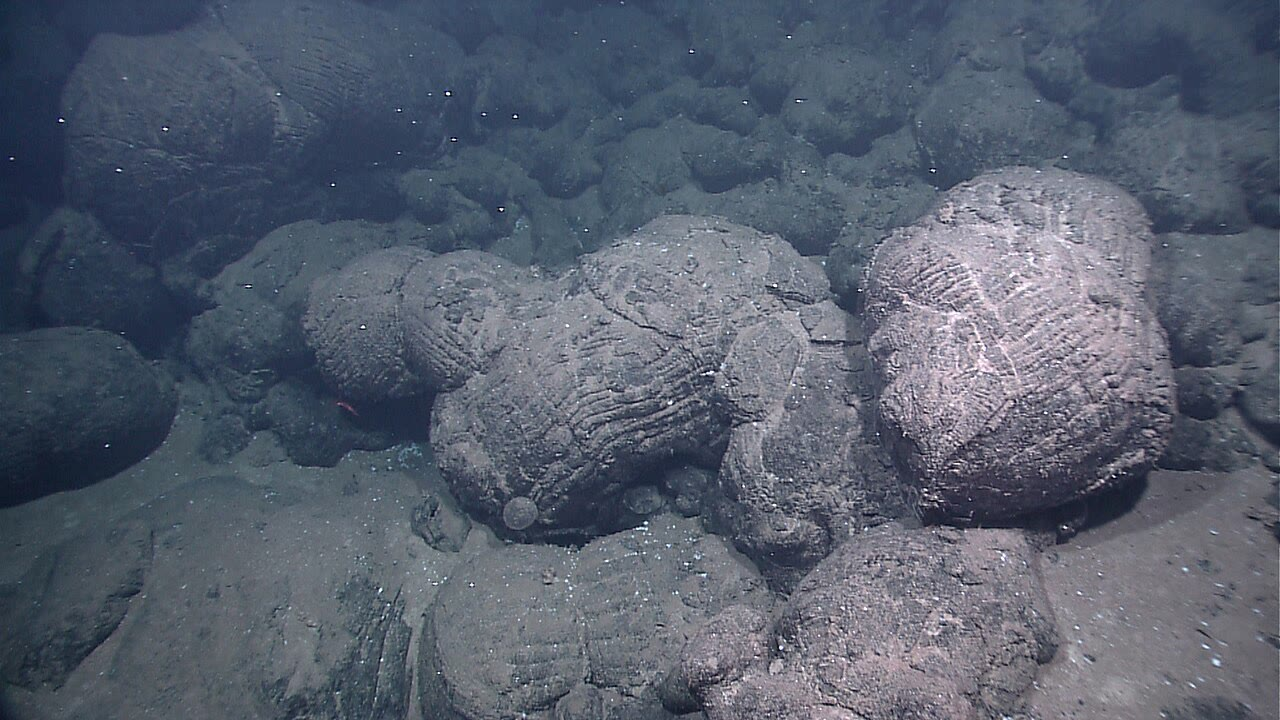
\includegraphics[width=0.8\linewidth]{images/book2/g11-noaa-pillow-lava.jpg}

{\small لابة وسائدية على صدع غالاباغوس، على عمق نحو 2500 متر،
صوّرتها مركبة يُتحكم فيها عن بعد عام 2011. وكل وسادة لسان
من اللابة تجمّد من الخارج لحظة التقائه بماء البحر البارد.
الصورة: برنامج «أوكيانوس إكسبلورر» التابع للإدارة الوطنية للمحيطات والغلاف الجوي (ملك عام).}
\end{omfigure}
% ledger: photo:g11-pillow-lava, whoi:alvin-1977 (depth of the rift floor)

\section{انصهار دون تسخين}

الوشاح تحت الظهرة \omterm{def:g11:ocean-ridges:peridotite}{بيريدوتيت} صلب، كما في كل مكان آخر. ومع ذلك يخرج منه
\qty{7}{km} من البازلت \omterm{def:g11:ocean-ridges:gabbro}{والغابرو}، أي صخر منصهر تجمّد. فمن أين
يأتي المصهور؟

\begin{definition}[الانصهار الجزئي؛ الانصهار بتخفيف الضغط]\label{def:g11:ocean-ridges:partial-melting}
\emph{الانصهار الجزئي}\index{انصهار جزئي} هو انصهار جزء
من الصخر فقط: فبعض معادنه، أو بعض مكوناتها، ينصهر، بينما
يبقى الباقي صلبًا.
و\emph{الانصهار بتخفيف الضغط}\index{انصهار بتخفيف الضغط} هو الانصهار الجزئي لصخر يصعد، فيقل
انضغاطه شيئًا فشيئًا، دون أن يُسخَّن.
\end{definition}

حين تتباعد صفيحتان، يصعد \omterm{def:g11:lithosphere-asthenosphere:lithosphere}{الغلاف اللدن} تحت الظهرة ليملأ
الفراغ. وهو يصعد أسرع من أن يفقد كثيرًا من حرارته، فلا تنخفض درجة حرارته
إلا بنحو \qty{0.45}{\celsius} لكل كيلومتر في طريقه إلى الأعلى. أما درجة
انصهاره، التي تتوقف على الضغط، فتنخفض أسرع بكثير: بنحو
\qty{3.9}{\celsius} لكل كيلومتر على عمق \qty{50}{km}. وعند عمق ما
يبلغ الصخر الصاعد درجة انصهاره فيبدأ بالانصهار، مع أن
أي حرارة لم تُضف إليه.
% ledger: katsura10:adiabat, hirschmann:solidus, white92:crust; computed in
% figdata/grade-11/ridge_melting.py (solidus_slope_50km 3.89)

\begin{method}[أين ينصهر الوشاح الصاعد؟]\label{met:g11:ocean-ridges:melting}
\begin{enumerate}
  \item اكتب درجة حرارة الصخر الصاعد عند كل عمق: درجة حرارته
        الكامنة (درجة الحرارة التي كانت ستكون له عند السطح)
        مضافًا إليها \qty{0.45}{\celsius} لكل كيلومتر من العمق.
  \item اكتب درجة انصهار الصخر عند كل عمق، انطلاقًا من
        الضغط عند ذلك العمق.
  \item جد العمق الذي تتساوى عنده الاثنتان. فأعمق منه يكون الصخر صلبًا؛
        وأقرب منه إلى السطح يكون منصهرًا جزئيًا.
\end{enumerate}
\end{method}

\begin{omfigure}
\begin{tikzpicture}
\begin{axis}[omrecord, omdepth, width=0.72\linewidth, height=6.4cm, xmin=1100, xmax=1700, ymin=0, ymax=150,
  xlabel={\foreignlanguage{arabic}{درجة الحرارة \babelsublr{(\unit{\celsius})}}}, ylabel={\foreignlanguage{arabic}{العمق \babelsublr{(\unit{km})}}},
  xticklabel style={/pgf/number format/set thousands separator={}}, clip=true]
% computed in figdata/grade-11/ridge_melting.py; ledger: katsura10:adiabat, hirschmann:solidus, data:prem
\addplot[omProp, line width=1.0pt] table[x=solidus, y=z] {figdata/out/grade-11-ridge_melting-curves.dat};
\addplot[omDef, line width=1.0pt] table[x=ad1300, y=z] {figdata/out/grade-11-ridge_melting-curves.dat};
\addplot[omDef, densely dashed, line width=0.9pt] table[x=ad1400, y=z] {figdata/out/grade-11-ridge_melting-curves.dat};
\addplot[only marks, mark=*, mark size=1.8pt, black] coordinates {(1324.3,54.1) (1438.3,85.0)};
\node[font=\scriptsize, anchor=east, align=right] at (axis cs:1316,62) {\foreignlanguage{arabic}{يبدأ الانصهار،}\\\foreignlanguage{arabic}{عند \babelsublr{\qty{54}{km}}}};
\node[font=\scriptsize, anchor=east] at (axis cs:1432,89) {\qty{85}{km}};
\node[font=\scriptsize, text=omProp, anchor=west, align=left] at (axis cs:1560,40) {درجة\\الانصهار};
\node[font=\scriptsize, text=omDef, anchor=east, align=right] at (axis cs:1318,128) {\foreignlanguage{arabic}{وشاح صاعد،}\\$T_p = \qty{1300}{\celsius}$};
\node[font=\scriptsize, text=omDef, anchor=west, align=left] at (axis cs:1476,140) {$T_p = \qty{1400}{\celsius}$};
\end{axis}
\end{tikzpicture}

{\small درجة حرارة صخر الوشاح الصاعد تحت ظهرة (بالأزرق) ودرجة
انصهاره (بالبرتقالي)، بدلالة العمق. فالصخر الذي درجة حرارته الكامنة
\qty{1300}{\celsius} يبدأ بالانصهار على عمق \qty{54}{km}؛ والصخر
الأسخن بمقدار \qty{100}{\celsius} (المتقطع) يبدأ منذ \qty{85}{km}. ودرجة
انصهار \omterm{def:g11:ocean-ridges:peridotite}{البيريدوتيت} الجاف مأخوذة من التجارب (هيرشمان، 2000).}
\end{omfigure}
% values: onset_1300_km 54.1, onset_1400_km 85.0, t_onset_1300 1324 (ridge_melting.py)

\begin{example}[عمق الانصهار]\label{ex:g11:ocean-ridges:onset}
في وشاح درجة حرارته الكامنة \qty{1300}{\celsius}، يكون الصخر الصاعد
عند $1300 + 0.45 \times 54 \approx \qty{1324}{\celsius}$ حين يبلغ
\qty{54}{km}، وهي درجة انصهاره عند ذلك العمق تمامًا: فيبدأ الانصهار
على عمق نحو \qty{54}{km}. وفوق ذلك العمق يستمر في الانصهار وهو يصعد.
\end{example}

لا ينصهر إلا كسر صغير من \omterm{def:g11:ocean-ridges:peridotite}{البيريدوتيت}، والمصهور ليس بيريدوتيتًا:
إنه بازلت. وتتجمع مصاهير البازلت من منطقة الانصهار كلها، التي تمتد
من عمق البداية حتى قاعدة القشرة؛ ولأنها أخف من الصخر
الصلب المحيط بها، فإنها تصعد إلى محور الظهرة. وهناك ينبثق جزء من الصهارة
لابةً، ويتجمد جزء في الشقوق التي صعد عبرها قواطعَ، ويتبلور جزء
ببطء في الأسفل \omterm{def:g11:ocean-ridges:gabbro}{غابرو}. \omterm{def:g11:ocean-ridges:peridotite}{والبيريدوتيت} الصلب المتبقي،
المستنزَف من بازلته، يصير الجزء الوشاحي من \omterm{def:g11:ocean-ridges:oceanic-lithosphere}{الغلاف الصخري المحيطي}.
% ledger: asimow01:morb, geo:basalt-ridges, white92:crust

حيث تعبر ظهرة منطقة من وشاح أسخن، حول بقعة ساخنة، يبدأ الانصهار
أعمق، وينصهر عمود أطول من الصخر ويُصنع بازلت أكثر: فهناك
يبلغ سمك القشرة نحو \qty{10}{km} بدلًا من 7. وعلى العكس، تحت الظهرات
البطيئة جدًا يجد الوشاح الصاعد وقتًا ليفقد حرارته، فينصهر أقل، ويصنع
قشرة رقيقة على غير المعتاد.
% ledger: white92:crust

\begin{omfigure}
\begin{tikzpicture}[font=\footnotesize]
  % schematic section across a ridge axis, not to scale
  \fill[omSea!45] (-6,0) rectangle (6,1.2);
  \fill[lith basalt] (-6,0) -- (-0.25,0) -- (-0.25,-0.35) -- (-6,-0.6) -- cycle;
  \fill[lith basalt] (6,0) -- (0.25,0) -- (0.25,-0.35) -- (6,-0.6) -- cycle;
  \fill[lith gabbro] (-6,-0.6) -- (-0.25,-0.35) -- (-0.25,-1.4) -- (-6,-1.6) -- cycle;
  \fill[lith gabbro] (6,-0.6) -- (0.25,-0.35) -- (0.25,-1.4) -- (6,-1.6) -- cycle;
  \fill[lith basalt] (-0.3,0) rectangle (0.3,-0.35);
  \fill[lith gabbro] (-0.3,-0.35) rectangle (0.3,-1.45);
  \fill[omProp!70] (-0.8,-0.75) .. controls (-0.4,-0.55) and (0.4,-0.55) .. (0.8,-0.75)
     .. controls (0.4,-0.95) and (-0.4,-0.95) .. (-0.8,-0.75);
  \fill[omProp!70] (-0.12,0) rectangle (0.12,-0.62);
  \fill[lith peridotite] (-6,-1.6) -- (-0.25,-1.4) -- (0.25,-1.4) -- (6,-1.6) -- (6,-5) -- (-6,-5) -- cycle;
  % melting region
  \fill[omProp!35] (-3.2,-1.5) -- (0,-4.0) -- (3.2,-1.5) -- cycle;
  \node[align=center] at (0,-2.95) {منطقة الانصهار};
  % isotherms deepening away from the axis
  \draw[omDef!70!black, densely dashed] (-6,-2.6) .. controls (-2.5,-2.0) and (-1,-1.1) .. (0,-1.0) .. controls (1,-1.1) and (2.5,-2.0) .. (6,-2.6);
  \draw[omDef!70!black, densely dashed] (-6,-4.2) .. controls (-3,-3.6) and (-1.2,-2.0) .. (0,-1.9) .. controls (1.2,-2.0) and (3,-3.6) .. (6,-4.2);
  \node[text=omDef!70!black, anchor=west] at (6.05,-2.6) {\qty{800}{\celsius}};
  \node[text=omDef!70!black, anchor=west] at (6.05,-4.2) {\qty{1200}{\celsius}};
  % flow arrows
  \draw[-{Stealth[length=5pt]}, line width=0.9pt] (0,-4.9) -- (0,-4.2);
  \draw[-{Stealth[length=5pt]}, line width=0.9pt] (-1.2,-4.8) .. controls (-1.0,-3.8) and (-2.2,-3.2) .. (-3.6,-3.2);
  \draw[-{Stealth[length=5pt]}, line width=0.9pt] (1.2,-4.8) .. controls (1.0,-3.8) and (2.2,-3.2) .. (3.6,-3.2);
  \draw[-{Stealth[length=5pt]}, line width=1.1pt] (-2,0.6) -- (-4,0.6);
  \draw[-{Stealth[length=5pt]}, line width=1.1pt] (2,0.6) -- (4,0.6);
  \node[anchor=south] at (-3,0.65) {صفيحة};
  \node[anchor=south] at (3,0.65) {صفيحة};
  \node[anchor=west] at (1.0,-0.8) {عدسة الصهارة};
  \node[anchor=east] at (-6.05,-0.3) {اللابات};
  \node[anchor=east] at (-6.05,-1.1) {الغابرو};
  \node[anchor=east] at (-6.05,-3.3) {الوشاح};
  \node[anchor=north] at (0,-5.05) {الوشاح يصعد وينصهر};
\end{tikzpicture}

{\small مقطع عبر محور ظهرة (رسم، ليس بمقياس رسم حقيقي). يصعد الوشاح
تحت المحور وينصهر جزئيًا؛ ويتجمع المصهور في عدسة صهارة
تحت المحور ويبني القشرة، التي تحملها الصفيحتان بعيدًا على
الجانبين. وتقع خطوط تساوي درجة الحرارة (المتقطعة) قريبة من السطح عند
المحور وأعمق فأعمق بالابتعاد عنه: \omterm{def:g11:lithosphere-asthenosphere:lithosphere}{فالغلاف الصخري} يزداد سمكًا وهو
يبرد.}
\end{omfigure}

\section{ظهرات سريعة وظهرات بطيئة}

تنفتح الظهرات بسرعات شديدة التفاوت. فإذا حُسبت من أقطاب الدوران في
\cref{ch:g11:plate-motions}، وُجد أن ظهرة شرق المحيط الهادئ عند \ang{30} جنوبًا تنفتح بمعدل
\qty{14.6}{cm} في السنة، وظهرة وسط الأطلسي عند دائرة العرض نفسها بمعدل
\qty{3.3}{cm} في السنة. وشكل المحور ليس واحدًا.
% ledger: nnr56:poles (computed in plate_velocities.py: epr30s_speed 145.8, atl30s_speed 32.7)

على امتداد الظهرات البطيئة يكون المحور واديًا عمقه 1 إلى \qty{2}{km} وعرضه 20 إلى
\qty{30}{km}. فالصهارة التي تبلغ المحور أقل من أن تملأ الفراغ
باستمرار: فيتمطط \omterm{def:g11:lithosphere-asthenosphere:lithosphere}{الغلاف الصخري} البارد الهش وينكسر على امتداد
صدوع.

\begin{definition}[الصدع العادي]\label{def:g11:ocean-ridges:normal-fault}
\emph{الصدع العادي}\index{صدع عادي} صدع مائل تحركت على امتداده
الكتلة الواقعة فوق مستوى الصدع إلى الأسفل بالنسبة إلى الكتلة الواقعة
تحته. وتتكوّن الصدوع العادية حيث تتمطط القشرة.
\end{definition}

وادي الظهرة البطيئة كتلة هبطت بين \omterm{def:g11:ocean-ridges:normal-fault}{صدوع عادية}
متقابلة؛ ويميل كلها تقريبًا نحو المحور. وتسمى هذه الكتلة الهابطة
بين \omterm{def:g11:ocean-ridges:normal-fault}{صدوع عادية} \emph{الغرابن}.
% ledger: buck05:valley, usgs:normal-fault

أما على امتداد الظهرات السريعة فتصل الصهارة بتواتر يكفي لملء الفراغ. فيكون المحور
مرتفعًا أملس لطيف الانحدار، فوق عدسة من الصهارة تقع تحته.
% ledger: buck05:valley, noaa:ridge

\begin{omfigure}
\begin{tikzpicture}[font=\footnotesize, x=0.24cm, y=0.9cm]
  % slow ridge: axial valley between normal faults (not to scale, vertical exaggeration)
  \begin{scope}
    \fill[omSea!45] (-15,-0.7) rectangle (15,1.6);
    \fill[lith basalt] (-15,0.9) -- (-9,0.9) -- (-8.5,0.2) -- (-6,0.2) -- (-5.5,-0.6) -- (5.5,-0.6)
      -- (6,0.2) -- (8.5,0.2) -- (9,0.9) -- (15,0.9) -- (15,-2.2) -- (-15,-2.2) -- cycle;
    \draw[black!70] (-15,0.9) -- (-9,0.9) -- (-8.5,0.2) -- (-6,0.2) -- (-5.5,-0.6) -- (5.5,-0.6)
      -- (6,0.2) -- (8.5,0.2) -- (9,0.9) -- (15,0.9);
    \draw[fault] (-9,0.9) -- (-7.4,-2.2);
    \draw[fault] (-6,0.2) -- (-4.6,-2.2);
    \draw[fault] (9,0.9) -- (7.4,-2.2);
    \draw[fault] (6,0.2) -- (4.6,-2.2);
    % slip arrows on the hanging walls (the axis side of each fault): down along the fault
    \foreach \x/\y/\s in {-7.9/-0.5/1, -5.0/-1.3/1, 7.9/-0.5/-1, 5.0/-1.3/-1} {
      \draw[-{Stealth[length=3pt]}, omProp, line width=0.8pt] (\x+0.9*\s,\y+0.45) -- ++(0.3*\s,-0.6);
    }
    \draw[-{Stealth[length=5pt]}, line width=1pt] (-11,1.25) -- (-14,1.25);
    \draw[-{Stealth[length=5pt]}, line width=1pt] (11,1.25) -- (14,1.25);
    \node at (0,-0.25) {الوادي المحوري};
    \node[anchor=north, align=center] at (0,-2.25) {ظهرة بطيئة: وادٍ\\بين صدوع عادية};
  \end{scope}
  % fast ridge
  \begin{scope}[xshift=8.2cm]
    \fill[omSea!45] (-15,0) rectangle (15,1.6);
    \fill[lith basalt] (-15,0.3) .. controls (-6,0.4) and (-2,0.9) .. (0,0.95) .. controls (2,0.9) and (6,0.4) .. (15,0.3)
      -- (15,-2.2) -- (-15,-2.2) -- cycle;
    \fill[omProp!75] (-2.5,-0.9) .. controls (-1,-0.7) and (1,-0.7) .. (2.5,-0.9) .. controls (1,-1.1) and (-1,-1.1) .. (-2.5,-0.9);
    \draw[black!70] (-15,0.3) .. controls (-6,0.4) and (-2,0.9) .. (0,0.95) .. controls (2,0.9) and (6,0.4) .. (15,0.3);
    \node[anchor=north] at (0,-1.25) {عدسة الصهارة};
    \draw[-{Stealth[length=5pt]}, line width=1pt] (-8,1.25) -- (-14,1.25);
    \draw[-{Stealth[length=5pt]}, line width=1pt] (8,1.25) -- (14,1.25);
    \node at (0,1.3) {المرتفع المحوري};
    \node[anchor=north, align=center] at (0,-2.25) {ظهرة سريعة: مرتفع لطيف\\فوق عدسة صهارة};
  \end{scope}
\end{tikzpicture}

{\small مقطعان عبر ظهرة بطيئة وأخرى سريعة (رسمان، ليسا بمقياس رسم حقيقي؛ والارتفاع
مبالغ فيه). في اليسار: الوادي المحوري لظهرة بطيئة، الذي يبلغ عمقه 1 إلى
\qty{2}{km}، قد هبط بين \omterm{def:g11:ocean-ridges:normal-fault}{صدوع عادية} تميل نحو المحور
(الأسهم البرتقالية: الكتل الواقعة فوق الصدوع تنزلق إلى الأسفل). في اليمين: ظهرة سريعة
ترتفع ارتفاعًا لطيفًا فوق عدسة من الصهارة.}
\end{omfigure}
% ledger: buck05:valley

\begin{example}[ظهرة بطيئة وأخرى سريعة]\label{ex:g11:ocean-ridges:rates}
في مليون سنة تصنع ظهرة شرق المحيط الهادئ عند \ang{30} جنوبًا
$\qty{14.6}{cm/yr} \times 10^6\ \text{سنة} = \qty{146}{km}$ من قاع
المحيط الجديد، \qty{73}{km} على كل جانب؛ وتصنع ظهرة وسط الأطلسي عند دائرة العرض نفسها
\qty{33}{km}، أي \qty{16.5}{km} على كل جانب. وقد دخلت البئر العميقة في شرق
المحيط الهادئ قشرة صُنعت بمعدل يزيد على \qty{20}{cm} في السنة، وهو من
أسرع معدلات التوسع المسجلة على الإطلاق.
\end{example}
% ledger: nnr56:poles (computed), iodp1256:section

\section{الفتحات الحرمائية}

القشرة الفتية عند المحور ساخنة، وتقطّعها الشقوق. فيشق ماء البحر
طريقه إليها.

\begin{definition}[الدوران الحرمائي؛ المدخنة السوداء]\label{def:g11:ocean-ridges:hydrothermal}
\emph{الدوران الحرمائي}\index{دوران حرمائي} هو جريان
ماء البحر نزولًا عبر شقوق \omterm{def:g11:ocean-ridges:oceanic-lithosphere}{القشرة المحيطية} الساخنة، حيث
تسخّنه الصهارة التي تحتها ويتفاعل مع الصخر، ثم صعودًا إلى قاع
البحر، حيث يخرج من \emph{الفتحات الحرمائية}. و\emph{المدخنة
السوداء}\index{مدخنة سوداء} فتحة يتدفق منها ماء شديد الحرارة يحمل
فلزات ذائبة؛ وحين يلتقي بماء البحر البارد، تترسب كبريتيدات الحديد
ومعادن أخرى على هيئة سحابة سوداء، وتبني مدخنة حول
الفتحة.
\end{definition}
% ledger: whoi:vents

يغادر ماء \omterm{def:g11:ocean-ridges:hydrothermal}{المدخنة السوداء} مدخنته عادة بنحو
\qty{350}{\celsius}، وقد تبلغ مياه الفتحات \qty{400}{\celsius}. ولا
تغلي، لأن كيلومترين ونصفًا من الماء تضغط عليها. وقد
تعلو المداخن أكثر من \qty{10}{m}. وحول الفتحات تستمد البكتيريا
طاقتها من كبريتيد الهيدروجين في ماء الفتحة، وتغذي الديدان الأنبوبية
والروبيان وبلح البحر: وعلى هذا عاشت محارات صدع غالاباغوس. ومعظم
الفتحات تقع على امتداد الظهرات وسط المحيطية.
% ledger: whoi:vents, whoi:alvin-1977

\begin{omfigure}
\begin{minipage}[c]{0.6\linewidth}\centering
\begin{tikzpicture}[font=\scriptsize, x=0.8cm, y=0.62cm]
  \fill[omSea!45] (0,0) rectangle (10,3);
  \fill[lith basalt] (0,0) rectangle (10,-4);
  \fill[omProp!70] (2,-4.6) .. controls (4,-4.0) and (6,-4.0) .. (8,-4.6) -- (8,-5) -- (2,-5) -- cycle;
  \node at (5,-4.7) {الصهارة};
  \fill[black!75] (4.7,0) -- (4.85,1.6) -- (5.15,1.6) -- (5.3,0) -- cycle;
  \fill[black!45, opacity=0.8] (5,1.7) circle (0.35) (5.2,2.2) circle (0.45) (4.9,2.7) circle (0.4);
  \draw[-{Stealth[length=4pt]}, omDef, line width=0.9pt] (1,0) .. controls (1,-2.5) and (2.5,-3.6) .. (4.2,-3.5);
  \draw[-{Stealth[length=4pt]}, omDef, line width=0.9pt] (9,0) .. controls (9,-2.5) and (7.5,-3.6) .. (5.8,-3.5);
  \draw[-{Stealth[length=4pt]}, omProp, line width=1.1pt] (5,-3.3) -- (5,-0.1);
  \node[align=center, text=omDef!80!black] at (1.6,1.0) {ماء البحر\\البارد يدخل};
  \node[align=left, anchor=west] at (5.6,1.4) {\foreignlanguage{arabic}{مدخنة سوداء،}\\\foreignlanguage{arabic}{نحو \babelsublr{\qty{350}{\celsius}}}};
  \node[align=left, anchor=west, text=omProp!80!black, fill=white, fill opacity=0.85, text opacity=1, inner sep=1.5pt] at (5.3,-1.8) {يسخن\\ويصعد};
\end{tikzpicture}
\end{minipage}\hfill
\begin{minipage}[c]{0.3\linewidth}\centering
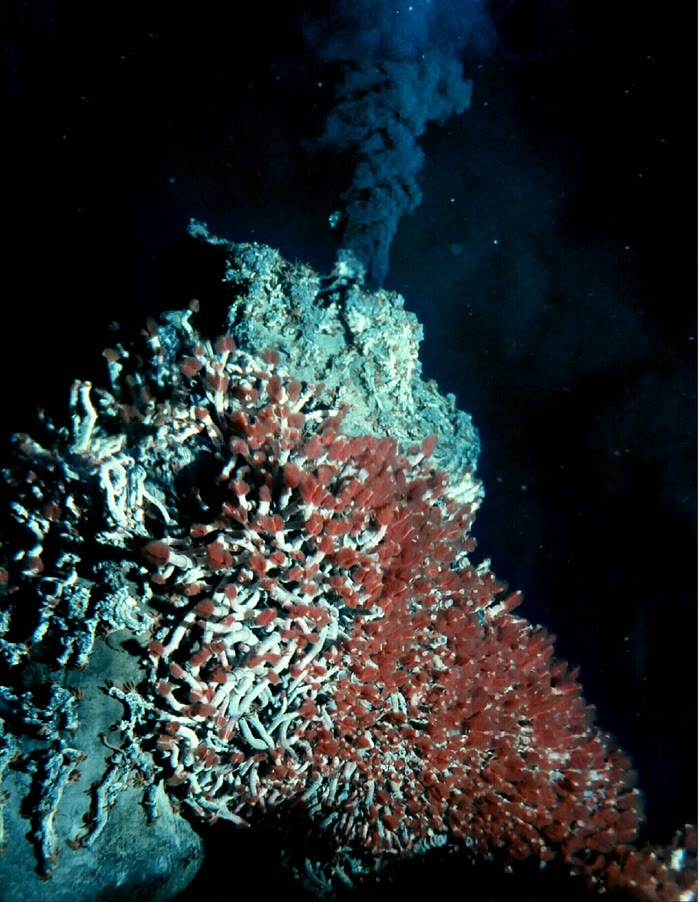
\includegraphics[width=\linewidth]{images/book2/g11-noaa-black-smoker.jpg}
\end{minipage}

{\small في اليمين: \omterm{def:g11:ocean-ridges:hydrothermal}{الدوران الحرمائي} عند محور ظهرة (رسم، ليس بمقياس
رسم حقيقي). في اليسار: \omterm{def:g11:ocean-ridges:hydrothermal}{مدخنة سوداء} على ظهرة خوان دي فوكا، مدخنتها مغطاة
بديدان أنبوبية ذات خياشيم حمراء؛ الصورة: جامعة واشنطن والإدارة الوطنية للمحيطات والغلاف الجوي
(ملك عام).}
\end{omfigure}
% ledger: whoi:vents, photo:g11-black-smoker

\begin{history}[\emph{«ألفين»} على صدع غالاباغوس، 1977]
بدأت البعثة، التي موّلتها المؤسسة الوطنية للعلوم، في
8~فبراير 1977 على متن سفينة البحث \emph{«كنور»}. فسجلت زلاجة الكاميرا ANGUS،
المسحوبة على عمق \qty{2500}{m} فوق الصدع، ارتفاعًا في درجة حرارة
الماء، وفي اللقطات نفسها أظهرت صورها مئات من المحار
الأبيض وأصداف بلح البحر البنية على اللابة. وفي الغطسة 713 للغواصة \emph{«ألفين»}، وجد
الجيولوجيان جاك كورليس وتيرد فان أندل ماءً بدرجة \qty{8}{\celsius}
يتلألأ خارجًا من الشقوق، ثم حتى \qty{17}{\celsius}، بينما كان الماء العميق
المحيط عند \qty{2}{\celsius}؛ وكانت محارات بيضاء يصل طولها إلى \qty{30}{cm}
تغطي مساحة عرضها نحو \qty{50}{m}. ولم يكن على متنها عالم أحياء: فقد
جاءت البعثة من أجل الماء الساخن، فوجدت مجتمعًا من الحيوانات لم
يتخيله أحد.
\end{history}
% ledger: whoi:alvin-1977

\section{التبرد، والتسمك، والغوص}

وهو يبتعد عن المحور، يبرد \omterm{def:g11:lithosphere-asthenosphere:lithosphere}{الغلاف الصخري} من أعلاه، عبر
المحيط البارد الذي فوقه. وتزداد الطبقة المبردة سمكًا مع الزمن: فيتسمك
\omterm{def:g11:lithosphere-asthenosphere:lithosphere}{الغلاف الصخري}، من بضعة كيلومترات عند المحور إلى نحو مئة
كيلومتر تحت القاع القديم. والصخر المبرد ينكمش ويزداد كثافة، فيطفو
\omterm{def:g11:lithosphere-asthenosphere:lithosphere}{الغلاف الصخري} أخفض على \omterm{def:g11:lithosphere-asthenosphere:lithosphere}{الغلاف اللدن} (\omterm{def:g11:lithosphere-asthenosphere:isostasy}{التوازن الأيزوستاتي}،
\cref{ch:g11:lithosphere-asthenosphere}): فيغوص قاع المحيط كلما تقدم في العمر.
وفي جسم يبرد بالتوصيل من سطحه، يزداد سمك
الطبقة المبردة بما يتناسب مع الجذر التربيعي للزمن.
% ledger: ps77:depth-age, rs09:lab

\begin{proposition}[عمق قاع المحيط بدلالة عمره]\label{prop:g11:ocean-ridges:depth-age}
في المتوسط، يقع قاع المحيط الذي عمره $t$ (بملايين السنين) على العمق
\[
  d(t) = 2500 + 350\sqrt{t} \quad \text{متر} \qquad (0 \le t \le 70),
\]
وللقاع الذي يزيد عمره على نحو 20 مليون سنة،
\[
  d(t) = 6400 - 3200\,e^{-t/62.8} \quad \text{متر}:
\]
فالقاع يغوص بسرعة ما دام فتيًا، ثم أبطأ فأبطأ، مقتربًا من
نحو \qty{6400}{m}. (مقبول دون برهان: فقد لاءم بارسونز وسكليتر عام 1977 الصيغتين مع أعماق
شمال المحيط الهادئ وشمال الأطلسي، بعد تصحيحها من وزن
رواسبهما.)
\end{proposition}
% ledger: ps77:depth-age

الجذر التربيعي يجعل القاع الفتي يغوص بسرعة: ففي مليون سنته الأولى
يغوص القاع \qty{350}{m}، وفي ملايين السنين الثلاثة التالية \qty{350}{m}
أخرى، وبين 16 و64 مليون سنة \qty{1400}{m}، أي بقدر ما غاص
في ملايين سنينه الستة عشر الأولى. أما القانون الأسي فيصف كيف يتوقف القاع
القديم عن الغوص: فهو يتصرف كأن للصفيحة المتبردة سمكًا ثابتًا،
نحو \qty{125}{km}.
% ledger: ps77:depth-age

\begin{omfigure}
\begin{tikzpicture}
\begin{axis}[omrecord, omdepth, width=0.82\linewidth, height=6.2cm, xmin=0, xmax=180, ymin=2000, ymax=6600,
  xlabel={\foreignlanguage{arabic}{عمر قاع المحيط بملايين السنين}}, ylabel={\foreignlanguage{arabic}{العمق \babelsublr{(\unit{m})}}},
  yticklabel style={/pgf/number format/set thousands separator={}},
  legend style={font=\scriptsize, at={(0.5,-0.32)}, anchor=north, legend columns=3, /tikz/every even column/.append style={column sep=6pt}}, legend cell align=left]
% computed in figdata/grade-11/depth_age.py; ledger: data:etopo1, data:b2-seafloor-age, ps77:depth-age
\addplot[only marks, mark=*, mark size=1.3pt, black!70, error bars/.cd, y dir=both, y explicit]
  table[x=age, y=depth, y error minus=em, y error plus=ep] {figdata/out/grade-11-depth_age-bins.dat};
\addplot[omProp, line width=1.0pt] table[x=age, y=depth] {figdata/out/grade-11-depth_age-sqrt.dat};
\addplot[omDef, line width=1.0pt, densely dashed] table[x=age, y=depth] {figdata/out/grade-11-depth_age-exp.dat};
\legend{{\foreignlanguage{arabic}{المقيس: الوسيط والنصف الأوسط}}, {$2500 + 350\sqrt{t}$}, {$6400 - 3200\,e^{-t/62.8}$}}
\end{axis}
\end{tikzpicture}

{\small عمق قاع المحيط بدلالة عمره: لكل نطاق عمري عرضه 5 ملايين
سنة، العمق الوسيط لكل خلايا محيطات العالم ذات الدرجة الواحدة،
ومدى النصف الأوسط منها. يتبع القاع الفتي قانون
الجذر التربيعي عن كثب؛ أما القاع الأقدم فيقع أقل عمقًا مما يعطيه القانونان، لأن
خلاياه تشمل رواسب وبراكين. البيانات: ETOPO1 (الإدارة الوطنية للمحيطات والغلاف الجوي)
وأعمار قاع المحيط لسيتون وآخرين (2020)؛ والقانونان لبارسونز وسكليتر
(1977).}
\end{omfigure}
% values (depth_age.py): median 2.5-5 Myr 3114 (law 3178), 60-65 Myr 4648 (law 5267), fit a 2727 b 255

تتفق الأعماق المقيسة للقاع الفتي مع القانون في حدود نحو
\qty{100}{m}. أما على القاع الأقدم فتقع الأوساط المقيسة أعلى من القانونين بعدة مئات من الأمتار.
فالقانونان يصفان عمق القاع نفسه، كأن
رواسبه قد أزيلت؛ أما الخلايا المقيسة فلا تزال تحمل رواسبها،
التي يزداد سمكها مع عمر القاع ويتجاوز كيلومترًا
على أقدم قاع في غرب شمال الأطلسي، وهي تشمل
جبالًا بحرية وهضابًا بركانية.
% ledger: ps77:depth-age; values from depth_age.py

\omterm{def:g11:ocean-ridges:oceanic-lithosphere}{فالغلاف الصخري المحيطي} القديم إذن سميك وبارد وكثيف. ويبيّن الفصل التالي
أنه قد يصير أكثف من \omterm{def:g11:lithosphere-asthenosphere:lithosphere}{الغلاف اللدن} الذي تحته، فيغوص
عائدًا إلى الوشاح (\cref{ch:g11:subduction-zones}).

\section{تمارين}

\begin{exercise}[$\star$]\label{exo:g11:ocean-ridges:1}
عرّف \omterm{def:g11:ocean-ridges:peridotite}{البيريدوتيت} \omterm{def:g11:ocean-ridges:gabbro}{والغابرو}. أيهما ينتمي إلى \omterm{def:g11:ocean-ridges:oceanic-lithosphere}{القشرة المحيطية}،
وأيهما إلى الوشاح؟ \omterm{def:g11:ocean-ridges:gabbro}{للغابرو} تركيب البازلت نفسه: فلماذا تكون
بلوراته أكبر بكثير؟
\end{exercise}

\begin{exercise}[$\star$]\label{exo:g11:ocean-ridges:2}
عدّد طبقات \omterm{def:g11:ocean-ridges:oceanic-lithosphere}{الغلاف الصخري المحيطي} من قاع البحر نزولًا. لقد بلغت البئر العميقة
في شرق المحيط الهادئ \qty{1507}{m} تحت قاع البحر: فما
الكسر الذي عبرته من قشرة سمكها \qty{7.1}{km}؟
\end{exercise}

\begin{exercise}[$\star$]\label{exo:g11:ocean-ridges:3}
باستعمال $d = 2500 + 350\sqrt{t}$، جد عمق قاع المحيط الذي عمره 0 و9 و25
مليون سنة.
\end{exercise}

\begin{exercise}[$\star$]\label{exo:g11:ocean-ridges:4}
عرّف \omterm{def:g11:ocean-ridges:normal-fault}{الصدع العادي}. عند ظهرة بطيئة، أي قوة تصنع \omterm{def:g11:ocean-ridges:normal-fault}{الصدوع العادية}،
وفي أي اتجاه تتحرك الكتل الواقعة فوق الصدوع؟
\end{exercise}

\begin{exercise}[$\star$]\label{exo:g11:ocean-ridges:5}
يخرج ماء \omterm{def:g11:ocean-ridges:hydrothermal}{المدخنة السوداء} بنحو \qty{350}{\celsius}. فلماذا لا
يغلي؟ وما «الدخان» الأسود؟
\end{exercise}

\begin{exercise}[$\star\star$]\label{exo:g11:ocean-ridges:6}
باستعمال شكل الانصهار: (1) على أي عمق يبدأ وشاح درجة حرارته الكامنة
\qty{1300}{\celsius} بالانصهار، وعند أي درجة حرارة؟ (2)
ووشاح أسخن بمقدار \qty{100}{\celsius}؟ (3) أيهما يصنع
القشرة الأسمك؟ ولماذا؟
\end{exercise}

\begin{exercise}[$\star\star$]\label{exo:g11:ocean-ridges:7}
صخر وشاحي صاعد درجة حرارته الكامنة \qty{1300}{\celsius} يكون عند
\qty{1345}{\celsius} على عمق \qty{100}{km}، حيث درجة انصهاره
\qty{1489}{\celsius}. (1) كم يقل عن درجة
انصهاره؟ (2) يبدأ بالانصهار عند \qty{54}{km}. فبكم درجة
لكل كيلومتر، في المتوسط، انغلقت الفجوة في الطريق إلى الأعلى؟ (3) هل
سُخّن الصخر؟
\end{exercise}

\begin{exercise}[$\star\star$]\label{exo:g11:ocean-ridges:8}
تنفتح ظهرة شرق المحيط الهادئ بمعدل \qty{14.6}{cm} في السنة عند \ang{30} جنوبًا،
وظهرة وسط الأطلسي بمعدل \qty{3.3}{cm} في السنة. بافتراض توسع متماثل، كم
تستغرق كل ظهرة لتصنع \qty{1000}{km} من القاع على جانب واحد؟
\end{exercise}

\begin{exercise}[$\star\star$]\label{exo:g11:ocean-ridges:9}
يبلغ طول الظهرات نحو \qty{65000}{km}. لنفترض أنها تنفتح في المتوسط بمعدل
\qty{5}{cm} في السنة وتصنع قشرة سمكها \qty{7.1}{km}. (1) ما مساحة قاع
المحيط الجديد التي تصنعها كل سنة؟ (2) وما حجم القشرة؟ (3) كم من الزمن
تحتاج لتصنع مساحة تساوي مساحة المحيطات،
\qty{3.6e8}{km^2}؟
\end{exercise}

\begin{exercise}[$\star\star$]\label{exo:g11:ocean-ridges:10}
عمق وادٍ محوري \qty{1.5}{km}. وقد هبط على امتداد صدعين عاديين
متقابلين، يميل كل منهما بزاوية \ang{60}. (1) بكم تحرك كل صدع
على امتداد مستواه؟ (2) كم تباعد الجانبان أفقيًا
بسبب الصدعين؟ (3) عرض الوادي \qty{25}{km}: فهل صنعه التصدع
وحده؟
\end{exercise}

\begin{exercise}[$\star\star$]\label{exo:g11:ocean-ridges:11}
باستعمال $d = 6400 - 3200\,e^{-t/62.8}$، جد عمق القاع الذي عمره 25 و100
مليون سنة، ومقدار ما يغوصه القاع بين هذين العمرين. وقارن
القيمة الأولى بقيمة قانون الجذر التربيعي.
\end{exercise}

\begin{exercise}[$\star\star\star$]\label{exo:g11:ocean-ridges:12}
يبرد عمود من الوشاح سمكه \qty{100}{km} بمقدار \qty{700}{\celsius} في
المتوسط. وينكمش الصخر بمقدار $\alpha = 3.2 \times 10^{-5}$ من طوله عن
كل درجة تبريد. (1) بكم يقصر العمود؟ (2) وبينما
يغوص، يملأ ماء البحر (\qty{1025}{kg/m^3}) الحيز الذي فوقه؛ ومع كثافة
للوشاح قدرها \qty{3380}{kg/m^3}، يجعل \omterm{def:g11:lithosphere-asthenosphere:isostasy}{التوازن الأيزوستاتي} القاع يغوص بمقدار
$s = \rho_m\,\alpha\,\Delta T\,L/(\rho_m - \rho_w)$. احسب $s$. (3) قارن
بالغوص الكلي الذي يسمح به القانون الأسي، من \qty{2500}{m} إلى
\qty{6400}{m}.
\end{exercise}

\begin{exercise}[$\star\star\star$]\label{exo:g11:ocean-ridges:13}
يبدأ الانصهار على عمق \qty{54}{km} في وشاح عند \qty{1300}{\celsius}،
وعلى عمق \qty{85}{km} في وشاح عند \qty{1400}{\celsius}؛ وفي كليهما يستمر الانصهار
حتى قاعدة القشرة، على عمق نحو \qty{7}{km}. (1) قارن طولي
عمودي الانصهار. (2) لو أعطى كل كيلومتر من الصخر الصاعد القدر نفسه
من المصهور، فكم يكون سمك القشرة فوق الوشاح الأسخن، إذا كانت
القشرة فوق الوشاح العادي \qty{7.1}{km}؟ (3) قارن بالسمك \qty{10.3}{km}
المقيس حيث تلتقي الظهرات بوشاح أسخن.
\end{exercise}

\begin{exercise}[$\star\star\star$]\label{exo:g11:ocean-ridges:14}
الأعماق الوسيطة المقيسة لقاع المحيط هي \qty{3114}{m} عند عمر
\num{3.75} مليون سنة، و\qty{4018}{m} عند \num{22.5}، و\qty{4465}{m} عند
\num{42.5}، و\qty{4648}{m} عند \num{62.5}. (1) احسب العمق الذي يعطيه
قانون الجذر التربيعي عند كل عمر، والفرق بينه وبين القياس. (2)
كيف يتغير الفرق مع العمر؟ (3) فسّره.
\end{exercise}

\begin{exercise}[$\star\star\star$]\label{exo:g11:ocean-ridges:15}
النقطة الحرجة للماء عند \qty{374}{\celsius} و\qty{22.064}{MPa}: فوق
هذا الضغط لا يغلي الماء عند أي درجة حرارة. (1) احسب
ضغط الماء على عمق \qty{2500}{m} (ماء البحر \qty{1025}{kg/m^3}،
$g = \qty{9.8}{m/s^2}$، مضافًا إليه ضغط الغلاف الجوي \qty{0.1}{MPa}). (2) هل يمكن
لماء فتحة أن يغلي على ذلك العمق، مهما كانت حرارته؟ (3) تحت أي عمق تقريبًا
يصح هذا لكل فتحة؟
\end{exercise}

\section{مسألة: حياة قطعة من قاع المحيط الهادئ}

\begin{problem}[{مسألة نهاية الأسبوع --- من الظهرة إلى المحيط العميق}]
\label{pb:g11:ocean-ridges:1}
% values: EPR 30 S full rate 145.8 mm/yr (plate_velocities.py, nnr56:poles); depth law
% ps77:depth-age; crust white92:crust; alpha ps77; densities data:prem; median 60-65 Myr
% 4648 m (depth_age.py)
تولد قطعة من قاع المحيط اليوم على ظهرة شرق المحيط الهادئ عند \ang{30}
جنوبًا، حيث تتباعد الصفيحتان الهادئية ونازكا بمعدل \qty{14.6}{cm} في السنة.
وهي تتحرك غربًا مع الصفيحة الهادئية. اعتبر التوسع متماثلًا،
والقشرة بسمك \qty{7.1}{km}، وقانون العمق $d = 2500 + 350\sqrt{t}$ مترًا
($t$ بملايين السنين).

\medskip
\noindent\textbf{الجزء الأول --- الولادة عند الظهرة.}
\begin{enumerate}
  \item ما نصف \omterm{def:g11:drift-to-spreading:spreading-rate}{معدل التوسع}، بالسنتيمترات في السنة وبالكيلومترات في كل
        مليون سنة؟
  \item على أي عمق تولد قطعة القاع؟
  \item عدّد الصخور التي تتكون منها، من قاع البحر حتى قاعدة
        \omterm{def:g11:lithosphere-asthenosphere:lithosphere}{الغلاف الصخري}.
  \item جاءت الصهارة التي صنعتها من الوشاح الذي تحتها. فسّر كيف
        انصهر الوشاح دون أن يُسخَّن.
  \item ما حجم القشرة الذي تصنعه هذه الظهرة في كل مليون سنة، على
        الجانبين، لكل كيلومتر من طولها؟
\end{enumerate}

\medskip
\noindent\textbf{الجزء الثاني --- الرحلة.}
\begin{enumerate}[resume]
  \item كم ستبعد القطعة عن الظهرة بعد 1 و4 و16 و64
        مليون سنة، إذا بقي المعدل كما هو؟
  \item كم من الزمن ستستغرق لتقطع \qty{2000}{km}؟
  \item لماذا قد تختلف المسافة الحقيقية بعد 64 مليون سنة عن
        جواب السؤال~6؟
  \item قرب الظهرة يدور ماء البحر عبر القشرة الفتية ويخرج
        من الفتحات. فلماذا يتوقف هذا الدوران على القاع القديم؟
  \item على أي صفيحة تسافر القطعة، ونحو أي نوع من حدود
        الصفائح تحملها تلك الصفيحة، على جانبها الغربي؟
\end{enumerate}

\medskip
\noindent\textbf{الجزء الثالث --- الغوص مع التقدم في العمر.}
\begin{enumerate}[resume]
  \item احسب عمقها عند 1 و4 و16 و64 مليون سنة.
  \item بكم تغوص خلال ملايين سنينها الستة عشر الأولى،
        وبين 16 و64 مليون سنة؟ علّق.
  \item عند أي عمر تبلغ عمق \qty{4000}{m}؟
  \item قارن عمقها عند 64 مليون سنة بالقانون الأسي،
        $6400 - 3200\,e^{-t/62.8}$.
  \item العمق الوسيط المقيس لقاع محيطي عمره 60 إلى 65 مليون سنة
        \qty{4648}{m}. فسّر الفرق.
\end{enumerate}

\medskip
\noindent\textbf{الجزء الرابع --- كثافتها ومصيرها.}
\begin{enumerate}[resume]
  \item عند 64 مليون سنة، اعتبر غلافها الصخري بسمك \qty{100}{km}
        وأبرد في المتوسط من \omterm{def:g11:lithosphere-asthenosphere:lithosphere}{الغلاف اللدن} بمقدار \qty{700}{\celsius}. ومع
        $\alpha = 3.2 \times 10^{-5}$ لكل درجة، بأي كسر صار
        الجزء الوشاحي أكثف؟ وانطلاقًا من \qty{3380}{kg/m^3}، ما
        كثافته؟
  \item سمك قشرتها \qty{7.1}{km}، وكثافتها
        \qty{2900}{kg/m^3}. احسب متوسط كثافة
        \omterm{def:g11:lithosphere-asthenosphere:lithosphere}{الغلاف الصخري} كله، وسمكه \qty{100}{km}.
  \item قارن \omterm{def:g11:lithosphere-asthenosphere:lithosphere}{بالغلاف اللدن} الذي تحتها، مأخوذًا بكثافة
        \qty{3380}{kg/m^3}.
  \item ماذا يمكن \omterm{def:g11:lithosphere-asthenosphere:lithosphere}{لغلاف صخري} كهذا أن يفعل حين يبلغ خندقًا؟
  \item استنتج: على أي عمق تقع هذه القطعة من القاع حين يبلغ عمرها 64
        مليون سنة؟
\end{enumerate}
\end{problem}
